\subsection{Distance metrics}

The following sections describe a range of different types of distance metrics,
that is, methods for measuring the distance between sequences.

\subsubsection{Edit distance}

One type of \emph{edit distance} is the \emph{Levenshtein
distance}~\cite{levenshtein}, which is a string metric for determining the
similarity between two sequences. It is defined to be the minimum number of
edits to transform the first sequence into the other~\cite[p.~52]{dong}.

The edit operations consists of \emph{insertions}, \emph{deletions} and
\emph{substitutions}. These operations are, respectively, inserting a letter,
removing a letter and changing one letter into another.

For example, the two sequences
\begin{center}
  \texttt{ACGT} \\
  \texttt{ACGGC}
\end{center}
would have a distance of 2 (e.g. substituting T for G and inserting a C). However,
there are some cases where the relevance of the distance is arguable. Consider
the sequences
\begin{center}
  \texttt{AACC} \\ %TODO: Reversals? Other example? Biology argument?
  \texttt{CCAA}
\end{center}
with a distance of 4. The two sequences actually have the maximal distance
possible even though one is just a reversal of the other. Since reversals of
substrings are commonly observed in sequence data~\cite{arslan}, this result
might not be appropriate.

A bottom-up dynamic programming version of the Levenshtein distance metric was
implemented and tested on real DNA/RNA data to evaluate its performance, and it
was clear that this algorithm is not suitable for large data sets, because it
would be infeasible to complete even a linear time clustering, in the number of
sequences to be clustered. The implementation could most likely be optimized
further, but because of the characteristics of an edit distance algorithm like
Levenshtein and because of the performance requirements for this project, it
was decided to not pursue further optimization and instead focus on other types
of algorithms. Furthermore, the Levenshtein distance penalizes reversals, i.e.
it results in an increased distance. %TODO: Data to show levenshtein is crap?

The Levenshtein distance can still be used for evaluation and benchmarking
against other metrics. The algorithm is attached in appendix
\ref{app:levenshtein_algorithm} and results from tests are shown in section
\ref{sec:results}.

As stated in \cite[pp.~1-2]{andoni}, ``The worst-case running time known for
this problem has not improved in three decades (..)'', specifically it states
that the running time of Levenshtein is $\mathcal{O}(d^2)$, where $d$ is the
length of the two sequences, and $\mathcal{O}(d^2/\log_2(d))$ for a constant
size alphabet. It further supports the conclusion that the running time of the
Levenshtein algorithm is too poor for the large data sets of the problem
domain.
% TODO: what if their lengths are different?

This lack of improvements of the performance of edit distance is one motivation
for the introduction of the concept of sequence alignment.

%The implemented dynamic programming solution has a running time of $O(nm)$,
%where $n$ and $m$ are the lengths of the sequences, and this running time seems
%to be inherent in this approach to measuring distance between sequences, as it
%needs to consider all possible edits to one sequence for each position in the
%other sequence. TODO: remove this?


\subsubsection{Sequence alignment}

\emph{Sequence alignment} is used in bioinformatics to identify regions of
similarity by aligning the characters of two or more sequences in a certain
manner. Besides shifting a sequence to a side, gaps can be inserted between
characters as well. A gap is represented with '-' and it indicates an insertion
in one sequence or a deletion from another sequence. This is called an
\emph{indel}, which is a contraction of the first letters from insertion and
deletion. If it is not have an indel and all characters in the column are same,
then it is a match. Otherwise, it is a mismatch~\cite[pp.~135-136]{dong}.

\begin{figure}[H]
  \centering
  \verb+ATGCAACGA+ \\
  \verb+ |||  |||+ \\
  \verb+-TGCG-CGA+
  \caption{Sequence alignment of `ATGCAACGA' and `TGCGCGA'}
  \label{fig:seq_alignment}
\end{figure}

Figure \ref{fig:seq_alignment} displays an alignment of two sequences. In
column 0 is an indel, in columns 1-3 are matches, in column 4 is a mismatch and
so forth. The vertical bar characters in the middle line, indicates matches.

% TODO: describe Needleman-Wunch
%The
%number of each type can then be used in a formula to calculate the similarity
%between the sequences. Note that more than two sequences can be aligned in a
%\emph{multiple sequence alignment}.
%
%There are many alignments and among those are optimal alignments, which are
%strived to be found or . Among those is an optimal alignment which is the one
%that is searched for.

Both \texttt{UCLUST} and the very recent project \texttt{VSEARCH} uses some
kind of sequence alignment for comparing sequences. \texttt{VSEARCH} uses a
parallelized version of the dynamic programming algorithm Needleman-Wunsch,
while \texttt{UCLUST} uses a heuristic procedure by default, but can be
instructed to use full dynamic programming with either the Needleman-Wunsch or
Smith-Waterman algorithm. However, this will make \texttt{UCLUST} much
slower.~\cite{vsearch} The heuristic algorithm used in \texttt{UCLUST} gives an
approximation of the optimal alignment for the purpose of increased
performance, but the alignment is not guaranteed to be optimal.

As opposed to \texttt{USEARCH}, \texttt{VSEARCH} is free and open-source
software and is designed for 64-bit processors, so it does not have the
limitation on usable memory that the free, 32-bit version of \texttt{USEARCH}
has.

Sequence alignment is still a computationally expensive operation and for
comparison of sequences with low similarity, the results of sequence alignment
are often poor. Additionally, as with the Levenshtein distance metric, sequence
alignment is very sensitive to the ordering of parts of sequences.
\emph{Alignment-free} sequence comparison methods strive to provide a measure
of sequence similarity while avoiding the costly computation that alignment
involves. Alignment-free comparison allows one to look at each of the sequences
independently, extracting some characteristics, or \emph{features}, of the each
sequence and then comparing these characteristics.  This can possibly reduce
the complexity of the comparison to linear time or better. One such
alignment-free method, is $k$-mer counting which will be presented and analyzed
in the following section.


\subsubsection{Feature based distance} \label{sec:kmer_distance}

A $k$-mer, or $k$-gram or simply a \emph{word}, is a subsequence of length
$k>0$ over some alphabet $\mathcal{A}$ of a sequence. An interesting feature of
a sequence is which $k$-mers occur in that sequence and how many times they
occur. This is called \emph{$k$-mer counting} and is a type of \emph{feature
based distance metric}.

The \emph{$d2$ distance metric} is a feature based distance metric, using
$k$-mers as the feature. The distance is calculated by counting the $k$-mers
occurring in two sequences, representing these occurrences as two vectors and
finally taking the Euclidean distance between these two
vectors~\cite[pp.~53-54]{dong}.

Let $c_x(w)$ be the number of times that a $k$-mer $w$ occurs in the sequence
$x$. Then the $d2$ distance between two sequences, $x$ and $y$, can be defined
as follows~\cite[pp.~1-2]{hazelhurst}
\begin{equation}
  d2_k(x,y) \eqdef \sqrt{\sum_{w \in K(x) \cup K(y)} (c_x(w) - c_y(w))^2}
\end{equation}
where $K(x)$ and $K(y)$ denotes the set of $k$-mers in $x$ and $y$,
respectively.

As an example, the two $2$-mer frequency vectors of the sequences
\begin{align*}
  S_1 &= ACTACAC \\
  S_2 &= ACAGAT
\end{align*}
over the alphabet $\mathcal{A} = \{A,C,T,G\}$, can be illustrated as follows:

\begin{table}[!h]
\centering
\scalebox{0.75}{
\begin{tabular}{c | c c c c c c c c c c c c c c c c}
        & AA & AC & AG & AT & CA & CC & CG & CT & GA & GC & GG & GT & TA & TC & TG & TT \\
  \hline
  $S_1$ &    &  3 &    &    &  1 &    &    &  1 &    &    &    &    &  1 &    &    &    \\
  \hline
  $S_2$ &    &  1 &  1 &  1 &  1 &    &    &    &  1 &    &    &    &    &    &    &    \\
\end{tabular}}
\end{table}

The Euclidean distance would then be calculated as
\begin{align*}
  d2_2(S_1, S_2)
    &= \sqrt{(3-1)^2 + (-1)^2 + (-1)^2 + (1-1)^2 + 1^2 + (-1)^2 + 1^2} \\
    &= \sqrt{9} = 3
\end{align*}

The first version of the $d2$ distance metric algorithm described above, is
shown in algorithm \ref{alg:d2_basic} and it has been implemented as well. The
substring method extracts up to $k$ characters beginning at index $i$ of the
string. This algorithm maintains a single frequency vector, as a map structure
to allow for large $k$ which results in a large number of possible different
$k$-mers. When iterating through the first sequence, $k$-mer counts are
incremented and when iterating through the second sequence, they are
decremented. Finally all the frequencies are squared and the square root of the
sum is returned, corresponding to the Euclidean distance between frequency
vectors for the two sequences.

\begin{algorithm}
  \caption{Basic \textsc{d2} distance metric}
  \label{alg:d2_basic}
  \begin{algorithmic}[1]
    \Require{$s$ and $t$ are DNA or RNA sequences and $k \in \mathbb{Z}^+$}
    \Statex
    \Function{d2}{$s, t, k$}
      \State initialize \texttt{freq\_map} of type \texttt{string $\to$ int} map
      \For{$i \gets 0$ to $length(s) - k$}
        \State \texttt{freq\_map}[$s$.substring($i$, $k$)]\texttt{++}
      \EndFor
      \For{$i \gets 0$ to $length(t) - k$}
        \State \texttt{freq\_map}[$t$.substring($i$, $k$)]\texttt{-{}-}
      \EndFor
      \State $total \gets 0$
      \ForAll{$e \in$ \texttt{freq\_map}}
        \State $total \gets total + e.value^2$
          \Comment{calculate the Euclidean distance}
      \EndFor
      \State \Return $\sqrt{total}$
    \EndFunction
  \end{algorithmic}
\end{algorithm}

To better support the measurement of distance between two sequences of
different length, but similar substrings, the concept of a \emph{window} can be
introduced. In this context, a window is a conceptual construction which gives
a view of fixed length substrings of two sequences. This window can then be
moved step by step over the two sequences, calculating the distance for each
position of the window and then using the lowest of those distances as the
resulting distance. In this way two sequences, where one is a prefix or postfix
of the other, will have zero distance. This concept is illustrated in figure
\ref{fig:d2_window_concept} where the blue box corresponds to the window, which
in this case has the length 10.

\begin{figure}[H]
\centering
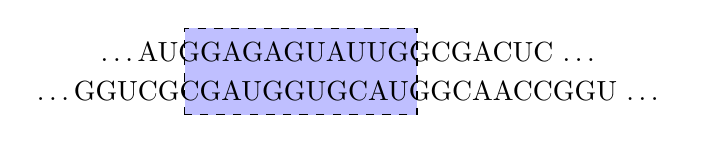
\begin{tikzpicture}
  \draw [fill=blue!25,dashed] (0,0.7) rectangle (2.95,1.8);
  \node at (2.1,1.5) {\dots AUGGAGAGUAUUGGCGACUC \dots};
  \node at (2.1,1.0) {\dots GGUCGCGAUGGUGCAUGGCAACCGGU \dots};
\end{tikzpicture}
\caption{Illustration of the concept of a window.}
\label{fig:d2_window_concept}
\end{figure}

For simplicity, the window size can be set equal to the size of the shortest of
the two sequences. Then the window only moves step by step over the longer of
the two sequences, while maintaining the position, and the $k$-mer counts, for
the shorter sequence.

Figure \ref{fig:d2_window_example} shows an example of this, where the $d2$
distance with the window is 0, since the first sequence is a prefix of the
other, while the $d2$ distance without a window gives a distance of 2.

\begin{figure}[H]
\centering
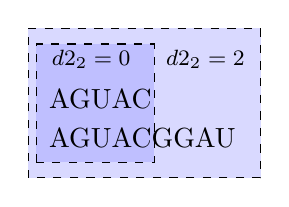
\begin{tikzpicture}
  \draw [fill=blue!15,dashed] (-0.45,0.5) rectangle (2.5,2.4);
  \draw [fill=blue!25,dashed] (-0.35,0.7) rectangle (1.15,2.2);
  \node at (1.0,1.5) {AGUAC\phantom{GGAU}};
  \node at (1.0,1.0) {AGUACGGAU};

  \node at (0.35, 2.0) {\footnotesize $d2_2 = 0$};
  \node at (1.8, 2.0) {\footnotesize $d2_2 = 2$};
\end{tikzpicture}
\caption{Example of difference in distance with window.}
\label{fig:d2_window_example}
\end{figure}

The $d2$ distance metric used in this project uses a window of length equal to
the shortest of the two sequences being compared. The distance between the
substrings in the initial, leftmost position of the window is calculated using
the basic \textsc{d2} algorithm described above.

The window then iterates over the longer sequence and calculates the new
distance between the substring of the longer sequence and the shorter sequence.
This calculation is done using a kind of forward differences method for
reducing the calculations to a few fixed operations for calculating the
distance in the next window from the distance in the current window. This
concept is described in~\cite{hazelhurst}.

% TODO: don't skip straight to Manhattan distance.

Let $|s|$ be the length of the shortest of the two sequences. To begin with
the, the $k$-mers in the first $|s|$ characters of each sequence are counted
and the \emph{Manhattan distance} between these two frequency vectors is
calculated using. The Manhattan distance is similar to the Euclidean distance
but with squaring replaced with absolute value and the square root omitted,
i.e.  for $u, v \in \mathbb{Z}^n$,

\begin{equation}
  d_{Manhattan} \eqdef \sum_{i=1}^{n} |u_i - v_i| \;.
\end{equation}

This distance metric was chosen for simplicity, to make the calculation of
distance in subsequent window positions easier, which also improves
performance, and since there is evidence in the literature that the Manhattan
distance generally is preferable to Euclidean distance for high dimensional
distance calculation~\cite{aggarwal}.

This distance is the distance between the subsequences in the first position of
the window. To calculate the distance in the following window, i.e. advancing
the window through the longer of the two sequences by one character, it is
decided which $k$-mers exit and enter the window, respectively, and then by
looking at whether the existing $k$-mer count in the frequency vector is
negative or positive, it can be decided whether the distance increases or
decreased by 2 or whether it stays the same. Subsequently, the frequency vector
is updated to reflect the change in the new window. The following illustrates
the idea of a window and $k$-mers exiting and entering the window:

%%\node at (4.3,1.5) {AUGGAGAGUAUUGGCGACUC\phantom{ACCGGU \dots}};
%%\node at (4.3,1.0) {GGUCGCGAUGGUGCAUGGCAACCGGU \dots};
%\begin{figure}[H]
%\centering
%\begin{tikzpicture}
%  \draw [fill=blue!25,dashed] (0,0.7) rectangle (3.95,1.8);
%  \node at (4.0,1.5) {ACTGATCGTAGCTAGCTAGTGTTG\phantom{TAGCTAAGCTTAGCTGATCG \dots}};
%  \node at (4.0,1.0) {ACGTAGATCGTGGATGGCTGATCGTAGCTAAGCTTAGCTGATCG \dots};
%\end{tikzpicture}
%\caption{Illustration of the concept of a window.}
%\label{fig:d2_forward_differences}
%\end{figure}

\begin{verbatim}
      |---- window ----------|
      ACTGATCGTAGCTAGCTAGTGTTG
      ACGTAGATCGTGGATGGCTGATCGTAGCTAAGCTTAGCTGATCG.....
      ^^^^                 ^^^^
      k-mer exiting        k-mer entering
\end{verbatim}
%TODO: Change figure to be consistent

The Manhattan distance can be a bad measurement for similarity, because it is very
dependent on the length of the shortest sequence (the length of the window),
the concept of the \emph{Jaccard index}~\cite{jaccard1901,jaccard1912}, or the
\emph{Jaccard similarity coefficient}, is used to normalize the distance to
a value in the interval $[0,1]$.

The Jaccard index of two sets $A$ and $B$ is defined as follows:
\begin{equation}
  J(A, B) \eqdef \frac{|A \cup B| - |A \cap B|}{|A \cup B|}
\end{equation}
 % TODO:  maybe actually Jaccard distance

In the context of $k$-mer frequencies, the union can be interpreted as the
total number of $k$-mers in the window in the two sequences, and the
intersection as the Manhattan distance in the window.
% TODO: "How is this related to distance measure", måske fint nok?

An algorithm \textsc{K-Dist} for calculating the $d2$ distance, using windows
and the Jaccard index, has been designed and implemented. This is the distance
metric used in the \texttt{klust} program.

\begin{algorithm}
  \caption{\textsc{K-Dist} algorithm}
  \label{alg:K-Dist}
  \begin{algorithmic}[1]
    \Require{$s$ and $t$ are DNA or RNA sequence, $k \in \mathbb{Z}^+$}
    \Statex
    \Function{d2}{$s, t, k$}
      \State set $s$ to the shortest sequence and $t$ to the longest sequence
      \State initialize array \texttt{kmers} of size $4^k$
      \State $cur\_dist \gets 0$
      \For{$i \gets 0$ to $length(s) - k$}
        \State \texttt{kmers}[$s$.substring($i$, $k$)]\texttt{++}
        \Comment{\parbox[t]{.3\linewidth}{$k$-mer counting}}
        \State \texttt{kmers}[$t$.substring($i$, $k$)]\texttt{-{}-}
      \EndFor
      \ForAll{$c \in$ \texttt{kmers}}
        \State $cur\_dist \gets cur\_dist + |c|$ \Comment{\parbox[t]{.3\linewidth}{Manhattan distance}}
      \EndFor
      \State $min\_dist \gets cur\_dist$
      \For{$i \gets 0$ to $length(t) - length(s)$} \Comment{\parbox[t]{.3\linewidth}{No. of windows}}
        \State \texttt{kmers}[$t$.substring($i$, $k$)]\texttt{-{}-}
        \State \texttt{kmers}[$t$.substring($length(s)-k+i+1$, $k$)]\texttt{++}
        \State update $cur\_dist$ to current Manhattan distance
        \State $min\_dist \gets min(min\_dist, cur\_dist)$
      \EndFor
          \State $total \gets 2(length(s)-k+1)$ \Comment{\parbox[t]{.3\linewidth}{Maximal distance}}
      \State \Return{$(total-min\_dist) / total$} \Comment{\parbox[t]{.3\linewidth}{Jaccard index}}
    \EndFunction
  \end{algorithmic}
\end{algorithm}
